\section{Outro}

\begin{frame}
  \begin{center}
    Part IV -- Outro
  \end{center}
\end{frame}

\subsection{Summary}

\begin{frame}{Conclusion: A framework for statistical testing}
  In this lecture, we introduced the concept of "hypothesis testing" as a way to use data obtained from an experiment to make conclusions about a population. Let's think back to the steps of this procedure:
  \bigskip

  \begin{itemize}
    \item Formulate the question of interest, and define the hypotheses;
    \item Define the minimally interesting effect;
    \item Define desired confidence and power for the test;
    \item Calculate required sample size;\hfill {\bf <- Future Lecture}
    \item Collect the data;
    \item Perform Statistial Analysis, and validate the assumptions;
    \item Draw conclusions and recommendations;
  \end{itemize}
  \bigskip

  In future lectures, we will study variations and special cases of this testing procedure;
\end{frame}

\begin{frame}{Recommended Reading}

  \begin{itemize}
    \item University of Guelph: "Statistical Significance vs Practical Significance: A tutorial."\url{https://atrium.lib.uoguelph.ca/xmlui/bitstream/handle/10214/1869/A_Statistical_versus_Practical_Significance.pdf?sequence=7}

    \item J.T. Mordkoff, "The Assumption(s) of Normality", 2016 \url{http://www2.psychology.uiowa.edu/faculty/mordkoff/GradStats/part\%201/I.07\%20normal.pdf}
  \end{itemize}

\end{frame}



\subsection{Scientist}
\begin{frame}{Florence Nightingale}{1820-1910 -- "The Lady with the Lamp"}
  \begin{columns}
    \column{.3\textwidth}
      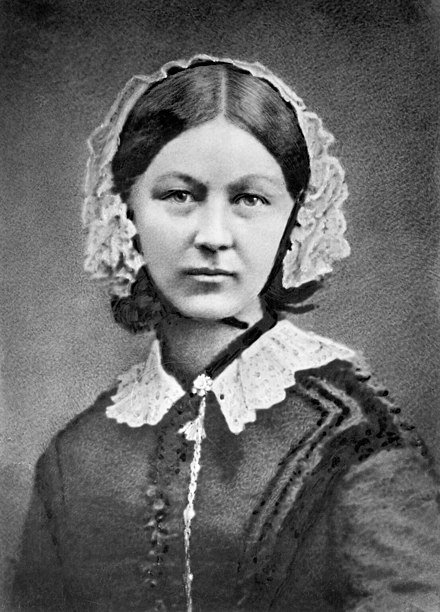
\includegraphics[width=\textwidth]{../img/florence}
    \column{.7\textwidth}
      Let's talk about a scientist who made great contributions to evidence-based medicine and descriptive statistics: {\bf Florence Nightingale}.\bigskip

      \begin{itemize}
        \item British nurse and mathematician;\medskip

        \item Born in 05/12/1820, her parents were opposed to her careers;
        \item She was driven, a prolific writer, and knew several languages;
        \medskip

        \item Gave great contributions for the professionalization of nursing;
      \end{itemize}
  \end{columns}
\end{frame}

\begin{frame}{Florence Nightingale}{Descriptive Statistics in Health}
  \begin{itemize}
    \item Implemented the use of {\bf hand washing} in hospitals for nurses:
    \item Pioneer of using of data visualization (infographics!) in medicine;
  \end{itemize}
  \begin{center}


    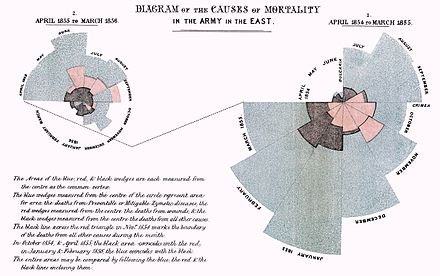
\includegraphics[width=.6\textwidth]{../img/florence_diagram}
  \end{center}
\end{frame}

\subsection{Fair Comparisons}
% - Fair Comparisons:

\begin{frame}{Experiment Design: Fair Comparisons}{A sombering example}

  Musgrave et al (preprint): several ML methods for metric learning perform exaclty the same when the hyperparameters are properly tuned for all methods.

  \begin{center}
    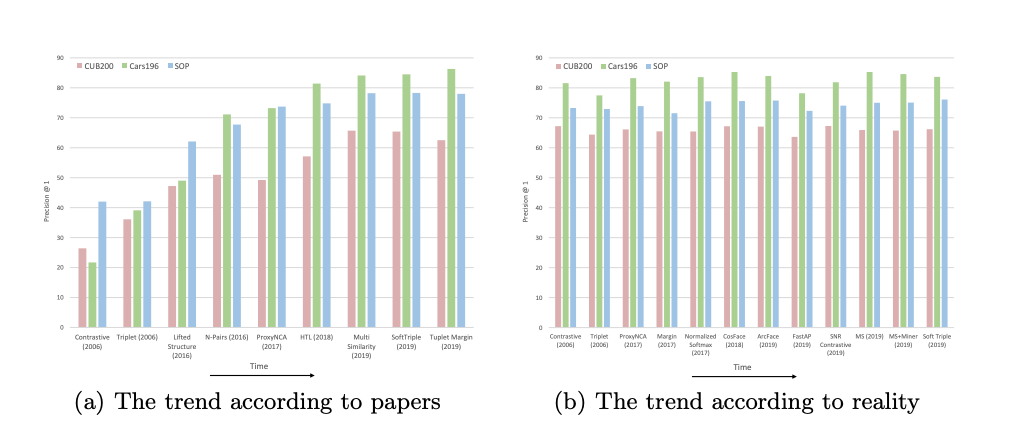
\includegraphics[width=.6\textwidth]{../img/musgrave_faircomparison}\\
    {\tiny Figure from Musgrave et al. "A Metric Learning Reality Check"}
    \ppagenote{Figure from Musgrave et al. "A Metric Learning Reality Check" \url{https://arxiv.org/pdf/2003.08505.pdf}}
  \end{center}

  \alert{Fair comparisons will help you avoid false conclusions!}
\end{frame}

\begin{frame}{Experiment Design: Fair Comparisons}{What are fair comparisons?}
  The definition of a {\bf fair} comparison, of course, depends on the field being studied and the experiment being conducted. In the comparison of algorithms in computer science, we can think of some points:
  \begin{itemize}
    \item Fine-tuning of algorithmic parameters;
    \item Discarding failed variations;\medskip
    \item Fine-tuning of the algorithm itself on the training data;
    \item Only comparing on data favorable to one of the algorithms;\medskip
    \item Coding with modern libraries vs old algorithms;
    \item Different computational environments;
    \item etc...
  \end{itemize}
\end{frame}
